\documentclass[letterpaper,12pt]{memoir}
\usepackage[utf8]{inputenc}
\usepackage[spanish,es-tabla]{babel}
\usepackage{amsfonts}
\usepackage{float}
\usepackage{mathptmx}
\usepackage[T1]{fontenc}
\usepackage[margin=1.3in]{geometry}
\usepackage{amsthm}
\usepackage{marvosym}
\usepackage{bm}
\usepackage{tikz}
\usepackage[tableaux]{prooftrees}

\linespread{1.3}


\usetikzlibrary{automata, positioning, arrows, fit}
\tikzset{
  ->,
  >=stealth',
  node distance=2cm,
  every state/.style={thick},
  initial text=$ $,
}

\renewcommand\qedsymbol{$\blacksquare$}

\theoremstyle{definition}
\newtheorem{definition}{Definición}[section]
\newtheorem*{thm}{Teorema}
\newtheorem*{solution}{Solución}
\newtheorem*{lem}{Lema}

\setlength\parindent{0pt}

\newcounter{paragraphnumber}
\newcommand{\para}{%
  \vspace{10pt}\noindent{\bfseries\refstepcounter{paragraphnumber}\theparagraphnumber.\quad}%
}

\setsecheadstyle{\large\bfseries}
\setsubsecheadstyle{\bfseries}

\setlength\parindent{0pt}

\pagenumbering{gobble}

%\usepackage[margin=1in]{geometry}

\usepackage{enumitem}
\setlist{nosep}

\usepackage{xcolor}

\usepackage{hyperref}
\hypersetup{
  colorlinks,
  linkcolor={red!50!black},
  citecolor={blue!50!black},
  urlcolor={green!50!black}
}

\usepackage{amssymb}
\usepackage{amsmath}

\begin{document}

\begin{center}
  {\large Lógica Computacional}\\
  \vspace{0.2cm}
  {\large\bfseries Examen 2}\\
  \vspace{0.2cm}
  {\large PCIC - UNAM}\\
  \vspace{0.5cm}
  {\itshape 1 de junio de 2020}\\
  \vspace{0.5cm}
  Diego de Jesús Isla López\\
  (\href{mailto:dislalopez@gmail.com}{\itshape dislalopez@gmail.com})\\
  (\href{mailto:diego.isla@comunidad.unam.mx}{\itshape diego.isla@comunidad.unam.mx})\\
\end{center}


\section*{Problema 1}

Eliminando la transición de \(s_2\) a \(s_1\), las únicas opciones para \(s_0\) son entrar a un ciclo ya sea desde \(s_2\) o desde \(s_3\), las cuales ambas contienen a \(p\), por lo que se sostiene.

\section*{Problema 2}

No se sostiene ya que el único caso en el que se cumple es al entrar en el ciclo de \(s_1\), donde solo aparece \(q\). En los demás caminos posibles desde \(s_0\) siempre aparece al menos una \(p\).

\section*{Problema 3}

\begin{itemize}
	\item \(\Box p\) y \(\Box\Box p\): Se construye un modelo con un mundo donde no se cumplen las dos al mismo tiempo:
	
	\begin{figure}[H]
		\centering
		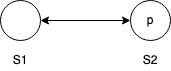
\includegraphics{world}
	\end{figure}

	En este modelo vemos que se cumple \(\Box p\) de \(s_1\) a \(s_2\); sin embargo debido a la transición de \(s_2\) a \(s_1\), no se cumple \(\Box\Box p\).
	
	\item \(\Box\neg p\) y \(\neg\diamond p\): Estas fórmulas son equivalentes por las reglas de DeMorgan, por lo tanto no es posible construir un modelo que contenga un mundo donde se cumpla solo alguna de las dos.
	
	\item \(\Box(p \land q)\) y \(\Box p \land \Box q\): Estas fórmulas son equivalentes por la regla de distributividad de \(\Box\) sobre \(\land\). Por lo tanto, no es posible construir un modelo que contenga un mundo donde se cumpla solo una de las dos fórmulas.
\end{itemize}

\section*{Problema 4}

\begin{itemize}
	\item Ningún mundo satisface esta fórmula. El mundo \(a\) cumple \(\Box\neg p\) pero no \(\Box\Box\neg p\). El mundo \(b\) no cumple ninguna de las dos y \(d\) solo cumple \(\Box\neg p\).
	\item Los mundos \(a\) y \(b\) cumplen esta fórmula.ya que desde ambos mundos es posible acceder a otros mundos donde existe al menos una \(q\) y otros donde no necesariamente se cumple \(q\).
	\item Los mundos \(a\),\(b\), \(e\) cumplen, ya que desde todos ellos se llega a algún vecino donde exista \(p\) o \(q\).
	\item Los mundos \(a\),\(b\),\(e\) cumplen. La fórmula es equivalente con la del punto anterior.
	\item Los mundos \(b\),\(d\),\(e\) cumplen.
	\item Todas los mundos cumplen. La fórmula alude a la presencia o no de \(p\), lo cual siempre se va a cumplir.
\end{itemize}


\end{document}